\section{Results}
\label{sec:results}

\begin{figure*}[!tp]
\centering
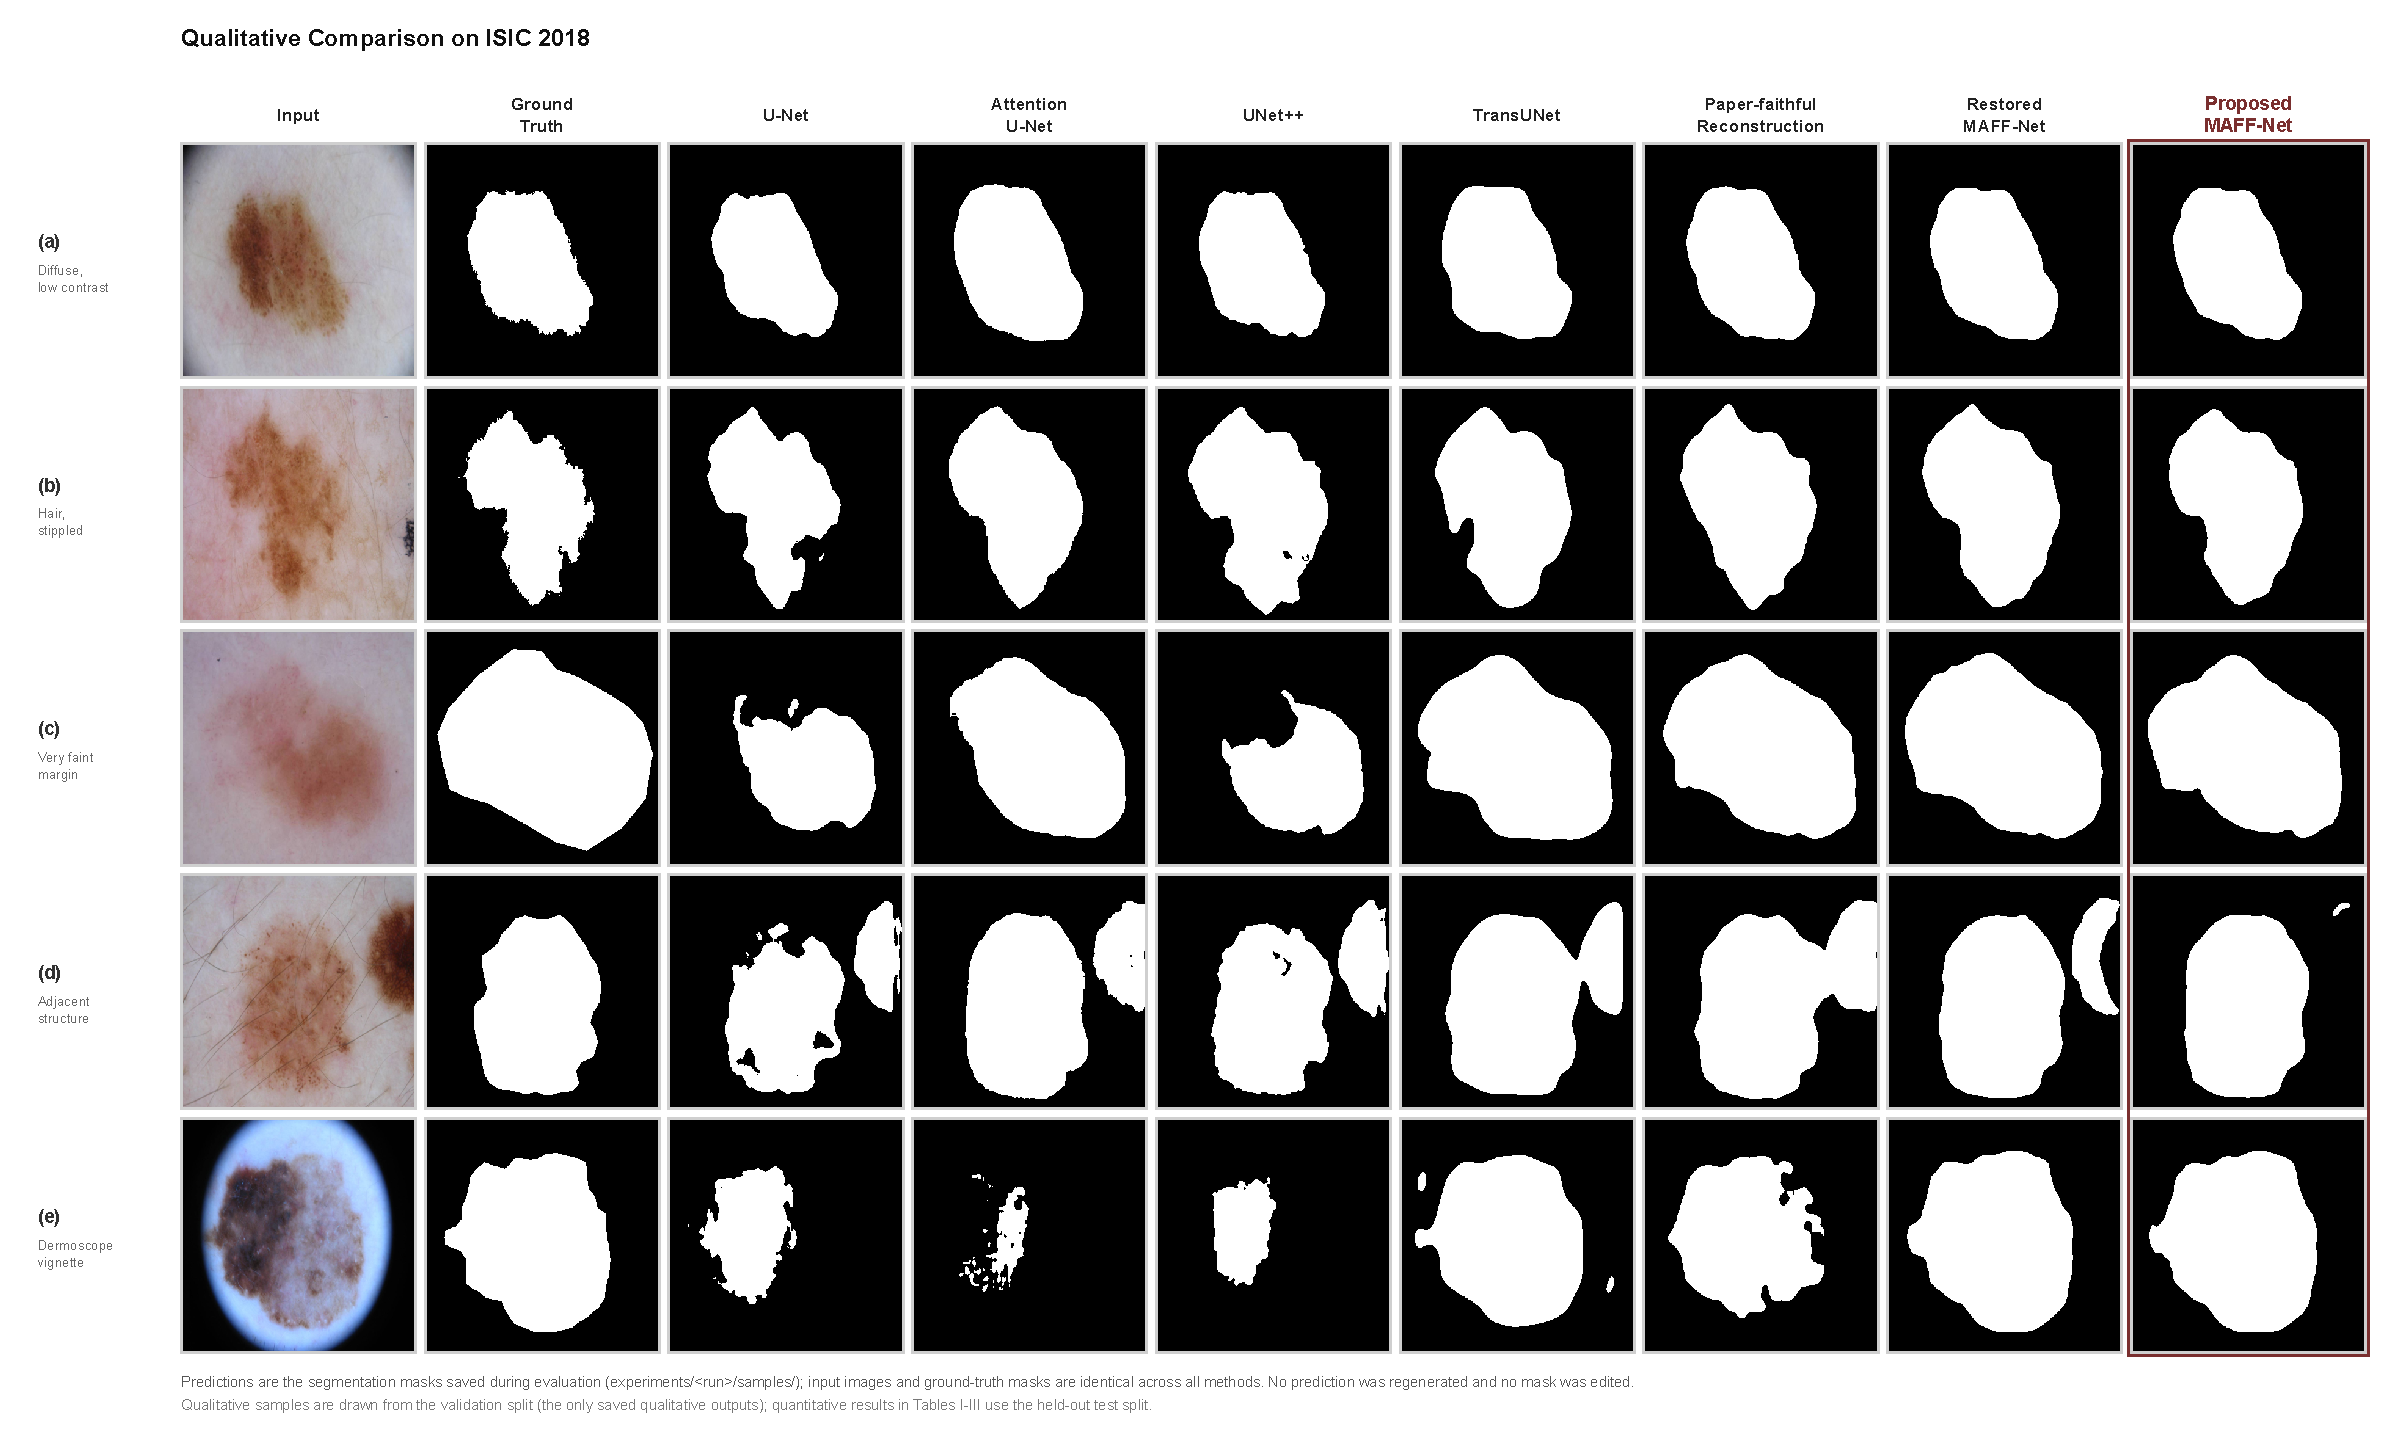
\includegraphics[width=\textwidth]{Figure4_QualitativeComparison.pdf}
\caption{Qualitative comparison on ISIC 2018. Each row is a test case and each
column a method, evaluated on identical input images and ground-truth masks; the
outlined column is the proposed model. Predictions are shown without
modification. The qualitative samples are drawn from the validation split.}
\label{fig:qualitative}
\end{figure*}

\subsection{Benchmark Comparison}

Table~\ref{tab:benchmark} reports the region-based segmentation performance of every evaluated model on the held-out test subsets of ISIC 2016, ISIC 2017, and ISIC 2018 --- the four baseline networks (U-Net, Attention U-Net, UNet++, and TransUNet) and the three members of the MAFF-Net family (the Paper-faithful Reconstruction, the Restored MAFF-Net, and the Proposed MAFF-Net). The Dice coefficient and the IoU are the principal indicators, with accuracy, sensitivity, and specificity reported alongside. Fig.~\ref{fig:region} presents these results graphically.

\begin{figure*}[!t]
\centering
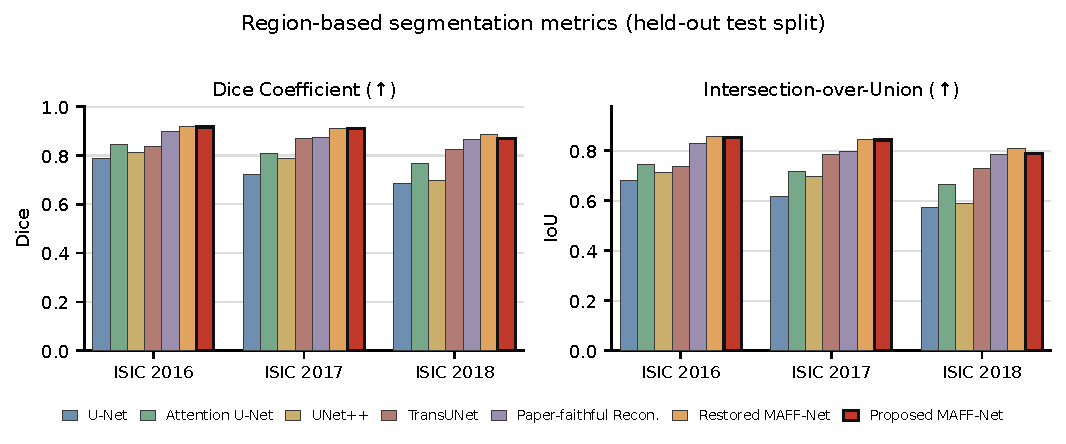
\includegraphics[width=\textwidth]{Figure5_RegionMetrics.pdf}
\caption{Region-based segmentation metrics (Dice and IoU) on the held-out test
splits of ISIC 2016, ISIC 2017, and ISIC 2018 for all evaluated models,
corresponding to Table~\ref{tab:benchmark}.}
\label{fig:region}
\end{figure*}

\begin{table*}[!t]
\centering
\caption{Region-based segmentation performance on the held-out test subsets of
ISIC 2016, ISIC 2017, and ISIC 2018. The highest value in each column, within
each dataset, is shown in bold.}
\label{tab:benchmark}
\setlength{\tabcolsep}{5pt}
\footnotesize
\begin{tabular}{llccccc}
\toprule
Dataset & Method & Dice & IoU & Accuracy & Sensitivity & Specificity \\
\midrule
\multirow{7}{*}{ISIC 2016}
 & U-Net & 0.7874 & 0.6808 & 0.8951 & 0.7649 & 0.9609 \\
 & Attention U-Net & 0.8466 & 0.7443 & 0.9178 & 0.8780 & 0.9495 \\
 & UNet++ & 0.8141 & 0.7140 & 0.9055 & 0.7996 & 0.9647 \\
 & TransUNet & 0.8365 & 0.7349 & 0.9161 & 0.8077 & \textbf{0.9700} \\
 & Paper-faithful Reconstruction & 0.8989 & 0.8264 & 0.9456 & 0.9096 & 0.9591 \\
 & Restored MAFF-Net & \textbf{0.9183} & \textbf{0.8555} & 0.9541 & \textbf{0.9414} & 0.9545 \\
 & Proposed MAFF-Net & 0.9169 & 0.8517 & \textbf{0.9548} & 0.9220 & 0.9689 \\
\midrule
\multirow{7}{*}{ISIC 2017}
 & U-Net & 0.7229 & 0.6152 & 0.9031 & 0.7211 & 0.9562 \\
 & Attention U-Net & 0.8097 & 0.7159 & 0.9331 & 0.8223 & 0.9737 \\
 & UNet++ & 0.7884 & 0.6959 & 0.9291 & 0.7776 & 0.9784 \\
 & TransUNet & 0.8683 & 0.7843 & 0.9561 & 0.8418 & \textbf{0.9870} \\
 & Paper-faithful Reconstruction & 0.8734 & 0.7975 & 0.9588 & 0.9123 & 0.9681 \\
 & Restored MAFF-Net & \textbf{0.9116} & \textbf{0.8447} & \textbf{0.9700} & \textbf{0.9171} & 0.9807 \\
 & Proposed MAFF-Net & 0.9096 & 0.8421 & 0.9682 & 0.9069 & 0.9842 \\
\midrule
\multirow{7}{*}{ISIC 2018}
 & U-Net & 0.6866 & 0.5714 & 0.8732 & 0.7766 & 0.8948 \\
 & Attention U-Net & 0.7662 & 0.6641 & 0.9207 & 0.8352 & 0.9497 \\
 & UNet++ & 0.6978 & 0.5878 & 0.8912 & 0.7692 & 0.9298 \\
 & TransUNet & 0.8259 & 0.7265 & 0.9259 & 0.8929 & 0.9315 \\
 & Paper-faithful Reconstruction & 0.8655 & 0.7855 & 0.9514 & 0.8779 & 0.9730 \\
 & Restored MAFF-Net & \textbf{0.8844} & \textbf{0.8080} & \textbf{0.9584} & \textbf{0.8973} & 0.9730 \\
 & Proposed MAFF-Net & 0.8701 & 0.7900 & 0.9493 & 0.8733 & \textbf{0.9768} \\
\bottomrule
\end{tabular}
\end{table*}

Among the baselines, the U-Net records the lowest Dice coefficient on all three datasets --- 0.7874, 0.7229, and 0.6866 on ISIC 2016, ISIC 2017, and ISIC 2018 --- with IoU values of 0.6808, 0.6152, and 0.5714. The ordering of the remaining baselines is not constant: on ISIC 2016 the Attention U-Net attains the highest baseline Dice coefficient, 0.8466, ahead of the TransUNet at 0.8365 and the UNet++ at 0.8141, whereas on ISIC 2017 and ISIC 2018 the TransUNet leads, at 0.8683 and 0.8259, followed by the Attention U-Net at 0.8097 and 0.7662 and the UNet++ at 0.7884 and 0.6978. The TransUNet is therefore the strongest baseline on two datasets and the Attention U-Net on the third.

All three members of the MAFF-Net family record higher Dice and IoU values than every baseline on every dataset. The narrowest margin occurs on ISIC 2017, where the Paper-faithful Reconstruction attains 0.8734 and 0.7975 against 0.8683 and 0.7843 for the TransUNet; the widest occurs on ISIC 2016, where the same lowest-scoring member attains a Dice coefficient of 0.8989 against 0.8466 for the Attention U-Net, a difference of 0.0523 (0.0396 on ISIC 2018). Relative to the strongest baseline on each dataset, the Proposed MAFF-Net records higher Dice coefficients by 0.0703, 0.0413, and 0.0442 on ISIC 2016, 2017, and 2018.

Within the family the ordering is consistent across all three datasets. The Restored MAFF-Net records the highest Dice coefficient and IoU of all evaluated models --- Dice 0.9183, 0.9116, and 0.8844 and IoU 0.8555, 0.8447, and 0.8080 on ISIC 2016, 2017, and 2018 --- and the Proposed MAFF-Net records the second-highest, with Dice 0.9169, 0.9096, and 0.8701 and IoU 0.8517, 0.8421, and 0.7900. The Dice differences between the Restored and Proposed MAFF-Net are 0.0014, 0.0020, and 0.0143 on the three datasets, and the Paper-faithful Reconstruction records the lowest Dice and IoU within the family throughout.

The remaining measures do not always follow the Dice ordering. The Proposed MAFF-Net attains the highest accuracy of all models on ISIC 2016, 0.9548 against 0.9541 for the Restored MAFF-Net, whereas the Restored MAFF-Net leads on ISIC 2017 and ISIC 2018, at 0.9700 and 0.9584. For specificity, the Proposed MAFF-Net exceeds the Restored MAFF-Net on all three datasets --- 0.9689 against 0.9545, 0.9842 against 0.9807, and 0.9768 against 0.9730 --- the last being the highest specificity on ISIC 2018, though the TransUNet attains the highest specificity of all models on ISIC 2016 and ISIC 2017, at 0.9700 and 0.9870. For sensitivity, the Restored MAFF-Net records the highest value within the family on all three datasets, at 0.9414, 0.9171, and 0.8973; on ISIC 2018 the TransUNet's 0.8929 exceeds both the Proposed MAFF-Net at 0.8733 and the Paper-faithful Reconstruction at 0.8779.

A consistent trend spans the three benchmarks: every model records its lowest Dice and IoU on ISIC 2018, and every model except the TransUNet its highest on ISIC 2016 (the TransUNet peaks on ISIC 2017). The spread between the strongest and weakest models is also widest on ISIC 2018, where Dice coefficients range from 0.6866 to 0.8844, against 0.7874 to 0.9183 on ISIC 2016. Each value corresponds to a single training run per configuration, so the narrower differences between models should be interpreted with corresponding caution. Finally, the Paper-faithful Reconstruction was trained without pretrained SAM2 weights; its values therefore characterise the reconstructed architecture under this study's training conditions and do not reproduce the results reported for the Original MAFF-Net.

\subsection{Boundary Evaluation}

In dermoscopic segmentation the practical value of a prediction depends heavily on the fidelity of the lesion margin, since the margin determines the measured extent of the lesion and is where annotation and prediction most often diverge. The region-overlap measures reported above, however, are dominated by the comparatively large and homogeneous interior: a contour displaced by a few pixels alters the overlap only marginally, so a model may attain a high overlap score while reproducing the margin imprecisely. Measures defined directly on the contour are therefore required. Table~\ref{tab:boundary} reports the three boundary-based measures of Section IV-C --- the 95th-percentile Hausdorff distance, the average symmetric surface distance, and the Boundary IoU --- for every model on the three datasets, and Fig.~\ref{fig:boundary} presents them graphically.

\begin{figure*}[!t]
\centering
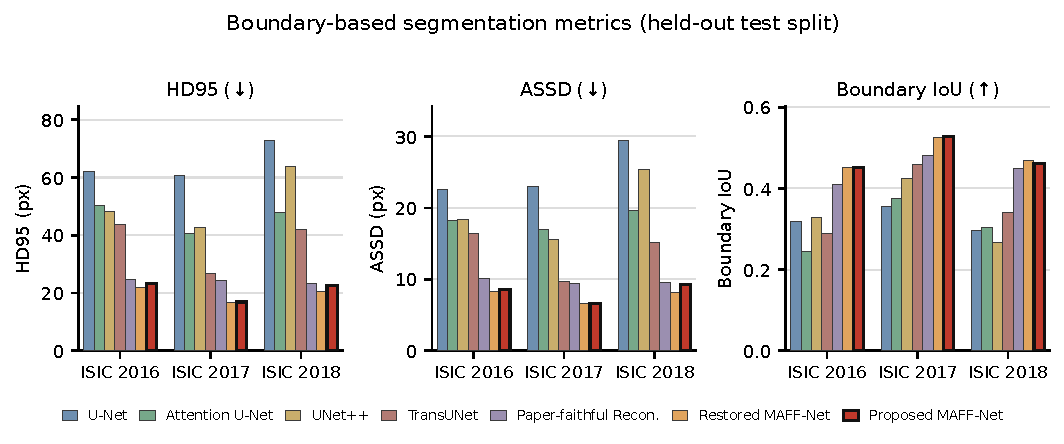
\includegraphics[width=\textwidth]{Figure6_BoundaryMetrics.pdf}
\caption{Boundary-based segmentation metrics (HD95, ASSD, and Boundary IoU) on
the held-out test splits, corresponding to Table~\ref{tab:boundary}. HD95 and
ASSD are in pixels of the $384\times384$ grid and lower is better; higher
Boundary IoU is better.}
\label{fig:boundary}
\end{figure*}

\begin{table*}[!t]
\centering
\caption{Boundary-based segmentation performance on the held-out test subsets of
ISIC 2016, ISIC 2017, and ISIC 2018. HD95 and ASSD are expressed in pixels of
the $384\times384$ evaluation grid, and lower values indicate closer agreement;
higher Boundary IoU values indicate closer agreement. The column
$n_{\mathrm{valid}}$ gives the number of images contributing to the distance
measures. The best value in each column, within each dataset, is shown in bold.}
\label{tab:boundary}
\setlength{\tabcolsep}{6pt}
\footnotesize
\begin{tabular}{llcccc}
\toprule
Dataset & Method & HD95 (px) & ASSD (px) & Boundary IoU & $n_{\mathrm{valid}}/n$ \\
\midrule
\multirow{7}{*}{ISIC 2016}
 & U-Net & 61.976 & 22.527 & 0.3195 & 192 / 192 \\
 & Attention U-Net & 50.465 & 18.221 & 0.2436 & 192 / 192 \\
 & UNet++ & 48.244 & 18.341 & 0.3283 & 190 / 192 \\
 & TransUNet & 43.779 & 16.368 & 0.2898 & 192 / 192 \\
 & Paper-faithful Reconstruction & 24.678 & 10.053 & 0.4101 & 191 / 192 \\
 & Restored MAFF-Net & \textbf{21.979} & \textbf{8.336} & \textbf{0.4518} & 192 / 192 \\
 & Proposed MAFF-Net & 23.329 & 8.510 & 0.4514 & 192 / 192 \\
\midrule
\multirow{7}{*}{ISIC 2017}
 & U-Net & 60.572 & 23.027 & 0.3560 & 194 / 200 \\
 & Attention U-Net & 40.745 & 17.004 & 0.3749 & 198 / 200 \\
 & UNet++ & 42.561 & 15.603 & 0.4244 & 197 / 200 \\
 & TransUNet & 26.750 & 9.710 & 0.4585 & 200 / 200 \\
 & Paper-faithful Reconstruction & 24.210 & 9.409 & 0.4806 & 200 / 200 \\
 & Restored MAFF-Net & \textbf{16.788} & \textbf{6.565} & 0.5255 & 200 / 200 \\
 & Proposed MAFF-Net & 16.869 & 6.645 & \textbf{0.5277} & 200 / 200 \\
\midrule
\multirow{7}{*}{ISIC 2018}
 & U-Net & 72.867 & 29.454 & 0.2958 & 388 / 392 \\
 & Attention U-Net & 47.746 & 19.645 & 0.3035 & 385 / 392 \\
 & UNet++ & 63.710 & 25.348 & 0.2672 & 383 / 392 \\
 & TransUNet & 41.836 & 15.092 & 0.3406 & 392 / 392 \\
 & Paper-faithful Reconstruction & 23.136 & 9.606 & 0.4491 & 390 / 392 \\
 & Restored MAFF-Net & \textbf{20.570} & \textbf{8.199} & \textbf{0.4701} & 392 / 392 \\
 & Proposed MAFF-Net & 22.554 & 9.240 & 0.4611 & 391 / 392 \\
\bottomrule
\end{tabular}
\end{table*}

The distance measures are undefined when a prediction contains no positive pixels; the affected images are excluded from the means and accounted for in the column $n_{\mathrm{valid}}$. Such cases arise for only a minority of images, predominantly among the baselines: the UNet++ produces an empty prediction for nine images of ISIC 2018 and the Attention U-Net for seven, whereas the TransUNet and the Restored MAFF-Net produce none on any dataset and the Proposed MAFF-Net produces one, on ISIC 2018. The Boundary IoU is defined for all images and computed over the complete test subsets.

All three members of the MAFF-Net family record lower HD95, lower ASSD, and higher Boundary IoU than every baseline on each of the three datasets --- the separation holding for all three measures simultaneously and on every dataset, not for an isolated measure or benchmark. Against the strongest baseline for each measure, the Proposed MAFF-Net reduces the HD95 from 43.779 to 23.329 pixels on ISIC 2016, from 26.750 to 16.869 on ISIC 2017, and from 41.836 to 22.554 on ISIC 2018, and the ASSD from 16.368 to 8.510, from 9.710 to 6.645, and from 15.092 to 9.240 pixels on the same datasets. Its Boundary IoU exceeds the highest baseline value by 0.1231, 0.0692, and 0.1205 on ISIC 2016, 2017, and 2018.

Within the family, the Restored MAFF-Net records the lowest HD95 and ASSD on all three datasets --- 21.979 and 8.336 pixels on ISIC 2016, 16.788 and 6.565 on ISIC 2017, and 20.570 and 8.199 on ISIC 2018 --- against 23.329 and 8.510, 16.869 and 6.645, and 22.554 and 9.240 pixels for the Proposed MAFF-Net. For the Boundary IoU the ordering is not uniform: the Proposed MAFF-Net records the highest value of all models on ISIC 2017, 0.5277 against 0.5255, while the Restored MAFF-Net is higher on ISIC 2016, 0.4518 against 0.4514, and ISIC 2018, 0.4701 against 0.4611. The Paper-faithful Reconstruction records the highest distances and lowest Boundary IoU within the family on all three datasets.

The orderings induced by the boundary measures do not coincide with those from region overlap, indicating that region overlap alone does not fully characterise contour quality. On ISIC 2016 the Attention U-Net records the highest Dice coefficient among the baselines yet the lowest Boundary IoU of all models, 0.2436, below the 0.3195 of the U-Net, which has the lowest Dice on that dataset. A comparable disagreement occurs on ISIC 2018, where the UNet++ records a higher Dice than the U-Net, 0.6978 against 0.6866, but a lower Boundary IoU, 0.2672 against 0.2958. Two models may therefore attain similar region overlap while differing appreciably in contour agreement, so the boundary measures provide information the region measures do not.

Three qualifications apply to the values in Table~\ref{tab:boundary}. Each corresponds to a single training run and no statistical testing was performed; the differences between closely ranked models, in particular within the MAFF-Net family, should be regarded as observations on these runs rather than established effects. The per-image dispersion is moreover large relative to the differences between neighbouring models: the standard deviation of the HD95 is of the same order as its mean for every model, ranging from 21.6 to 30.3 pixels within the MAFF-Net family and from 33.9 to 64.8 pixels for the baselines. Finally, as noted in Section IV-C, HD95 and ASSD are in pixels of the 384$\times$384 grid rather than physical units, so they are comparable among the models here but not with distances reported in millimetres elsewhere.

\subsection{Architecture Ablation}

The three components introduced in this work --- the Frequency Branch, the Feature Alignment Module, and the Gated Fusion Module --- were examined by the leave-one-out ablation of Section IV-D, in which each is disabled in turn while the rest of the network and the training configuration are held fixed. The study was conducted on ISIC 2018. Table~\ref{tab:ablation} reports both the region-based and boundary-based measures for the complete model and the three ablated configurations, so that the two families may be considered together.

\begin{table*}[!t]
\centering
\caption{Leave-one-out architecture ablation on the ISIC 2018 test subset. HD95
and ASSD are expressed in pixels of the $384\times384$ evaluation grid, and lower
values indicate closer agreement; higher Dice, IoU, accuracy, and Boundary IoU
values indicate closer agreement. The best value in each column is shown in
bold.}
\label{tab:ablation}
\setlength{\tabcolsep}{6pt}
\small
\begin{tabular}{lcccccc}
\toprule
Configuration & Dice & IoU & Accuracy & HD95 (px) & ASSD (px) & Boundary IoU \\
\midrule
Full Proposed MAFF-Net & 0.8701 & 0.7900 & 0.9493 & \textbf{22.554} & \textbf{9.240} & \textbf{0.4611} \\
without Frequency Branch & 0.8708 & 0.7868 & 0.9496 & 23.574 & 9.546 & 0.4416 \\
without Feature Alignment Module & 0.8649 & 0.7811 & 0.9502 & 23.676 & 9.869 & 0.4326 \\
without Gated Fusion Module & \textbf{0.8725} & \textbf{0.7907} & \textbf{0.9520} & 25.546 & 9.488 & 0.4508 \\
\bottomrule
\end{tabular}
\end{table*}

On the boundary-based measures, the complete Proposed MAFF-Net records the best value of the four configurations on all three: the lowest HD95 at 22.554 pixels, the lowest ASSD at 9.240 pixels, and the highest Boundary IoU at 0.4611. Disabling any one component degrades all three simultaneously: removing the Frequency Branch increases the HD95 by 1.020 pixels and the ASSD by 0.306 and reduces the Boundary IoU by 0.0196; removing the Feature Alignment Module increases them by 1.121 and 0.629 pixels and reduces the Boundary IoU by 0.0286; and removing the Gated Fusion Module increases them by 2.992 and 0.248 pixels and reduces the Boundary IoU by 0.0103. No single component accounts for the whole difference, and the ordering depends on the measure: the largest HD95 increase follows removal of the Gated Fusion Module, the largest ASSD increase and Boundary IoU reduction that of the Feature Alignment Module.

The region-based measures do not separate the four configurations in the same way, and do not favour the complete model. The Dice coefficient varies from 0.8649 to 0.8725, a spread of 0.0076, and the complete model, at 0.8701, does not record the highest value: the configuration without the Gated Fusion Module records the highest Dice at 0.8725, IoU at 0.7907, and accuracy at 0.9520, while the complete model records the lowest accuracy of the four, 0.9493. The only configuration whose Dice falls below the complete model's is the one without the Feature Alignment Module, at 0.8649. The present evidence therefore does not support the proposition that these components improve region overlap, and no such claim is made.

Considered together, the two families indicate that the effect of the three components is confined to the fidelity of the predicted contour rather than the extent of the predicted region. This is consistent with Section V-B, that region overlap is comparatively insensitive to contour displacements: a configuration may reproduce the lesion area to within a small Dice difference while agreeing less closely with the reference contour. On this evidence, the architectural contribution of the present work is accordingly an improvement in boundary fidelity, not in region-overlap performance.

Three qualifications delimit these observations. Each configuration was trained once, with a single experimental seed, and no repeated runs or statistical testing were performed; the differences in Table~\ref{tab:ablation} are therefore observations on these particular runs, not established as statistically significant. The magnitudes are moreover small relative to the per-image dispersion noted in Section V-B, which further limits the weight individual differences can bear. Finally, the study was conducted on ISIC 2018 alone, so the consistency of these observations across the other two datasets is not established here.

\subsection{Qualitative Analysis}

The quantitative measures above summarise agreement over entire test subsets and do not indicate how the predicted contours depart from the reference annotations. Fig.~\ref{fig:qualitative} accordingly presents representative segmentation results on ISIC 2018 for the baselines and the members of the MAFF-Net family, using the same images and annotations for every method so that the predictions may be compared directly. The cases shown are illustrative examples spanning the difficulties of dermoscopic imaging, intended to complement rather than substantiate the quantitative findings.

A characteristic common to all methods concerns the fine structure of the contour. The reference annotations exhibit pixel-level serration along the lesion margin, whereas the predictions of every method, baseline and MAFF-Net variant alike, are comparatively smooth at that scale. None of the models reproduces the finest irregularities of the manual delineation, so the differences observed between methods concern the coarser shape of the contour rather than its fine detail. This applies uniformly and should be borne in mind when assessing the visual results.

For lesions of low contrast and diffuse margin, in which the pigmented region fades gradually into the surrounding skin, the methods differ chiefly in how closely the predicted contour follows the reference outline. The baselines recover the overall extent of such lesions, but their contours tend towards rounded, approximately convex forms --- most evidently the TransUNet, which reproduces the lesion as a compact convex region and does not follow the concavities in the reference outline. The Restored and Proposed MAFF-Net follow the asymmetric form of the reference more closely, reproducing indentations along the margin and the lesion's elongation towards one side, though their contours remain smoother than the annotation at the finest scale.

The methods also differ in the internal consistency of the predicted regions. In several cases examined, the convolutional baselines contain small unsegmented cavities within the lesion interior and isolated fragments detached from the principal region, giving the boundary a broken appearance in places. The MAFF-Net family in the same cases forms closed regions without interior cavities, returning the lesion as a single connected component with a continuous margin. The contours produced by the MAFF-Net variants are correspondingly more regular --- exhibiting fewer isolated fragments and discontinuities, rather than more detail.

The cases containing structures adjacent to the target lesion are the most discriminating. In one, the image is traversed by dense hair and contains a second, darker pigmented structure near the border, excluded by the reference annotation. The U-Net, UNet++, and Attention U-Net each segment this adjacent structure as an additional region, and the TransUNet segments it and connects it to the target lesion, returning the two as one continuous region. The Restored and Proposed MAFF-Net confine the segmentation to the target lesion and return its margin as a closed contour; a residual response to the adjacent structure remains in both, larger for the Restored MAFF-Net and reduced to a small isolated fragment for the Proposed MAFF-Net. The dense hair overlying the lesion does not visibly fragment the MAFF-Net contours, whereas several baselines' margins are locally irregular where the hair traverses.

These observations are subject to clear limitations. They rest on a small number of saved examples per model, drawn from the validation split rather than the test subsets on which the quantitative results were computed, and derive from single training runs. They are consequently illustrative of the models' behaviour on the cases shown, not a representative sample, and do not constitute independent evidence of the differences reported in Sections V-A to V-C. The visual comparison is presented for interpretive value only, and the quantitative measures remain the basis for the comparisons drawn in this work.
